
% License:
% CC BY-NC-SA 3.0 (http://creativecommons.org/licenses/by-nc-sa/3.0/)
%
%%%%%%%%%%%%%%%%%%%%%%%%%%%%%%%%%%%%%%%%%

%----------------------------------------------------------------------------------------
%	PACKAGES AND OTHER DOCUMENT CONFIGURATIONS
%----------------------------------------------------------------------------------------

\documentclass[paper=a4, fontsize=11pt]{scrartcl} % A4 paper and 11pt font size

\usepackage[T1]{fontenc} % Use 8-bit encoding that has 256 glyphs
\usepackage{fourier} % Use the Adobe Utopia font for the document - comment this line to return to the LaTeX default
\usepackage[english]{babel} % English language/hyphenation
\usepackage{amsmath,amsfonts,amsthm} % Math packages
\usepackage{lipsum} % Used for inserting dummy 'Lorem ipsum' text into the template

\usepackage{caption}
\usepackage{subcaption}
\usepackage{graphicx}

\usepackage{float}

\usepackage{blindtext} %for enumarations

\usepackage[]{hyperref}  %link collor

\usepackage{xargs}                      % Use more than one optional parameter in a new commands
\usepackage[pdftex,dvipsnames]{xcolor}  % Coloured text etc.
% 
\usepackage[colorinlistoftodos,prependcaption,textsize=tiny]{todonotes}
\newcommandx{\unsure}[2][1=]{\todo[linecolor=red,backgroundcolor=red!25,bordercolor=red,#1]{#2}}
\newcommandx{\change}[2][1=]{\todo[linecolor=blue,backgroundcolor=blue!25,bordercolor=blue,#1]{#2}}
\newcommandx{\info}[2][1=]{\todo[linecolor=OliveGreen,backgroundcolor=OliveGreen!25,bordercolor=OliveGreen,#1]{#2}}
\newcommandx{\improvement}[2][1=]{\todo[linecolor=Plum,backgroundcolor=Plum!25,bordercolor=Plum,#1]{#2}}
\newcommandx{\thiswillnotshow}[2][1=]{\todo[disable,#1]{#2}}


%talbe layout to the right
%\usepackage[labelfont=bf]{caption}
%\captionsetup[table]{labelsep=space,justification=raggedright,singlelinecheck=off}
%\captionsetup[figure]{labelsep=quad}

\usepackage{sectsty} % Allows customizing section commands
\allsectionsfont{\centering \normalfont\scshape} % Make all sections centered, the default font and small caps

\usepackage{fancyhdr} % Custom headers and footers
\usepackage{register} % Custom headers and footers
\pagestyle{fancyplain} % Makes all pages in the document conform to the custom headers and footers
\fancyhead{} % No page header - if you want one, create it in the same way as the footers below
\fancyfoot[L]{} % Empty left footer
\fancyfoot[C]{} % Empty center footer
\fancyfoot[R]{\thepage} % Page numbering for right footer
\renewcommand{\headrulewidth}{0pt} % Remove header underlines
\renewcommand{\footrulewidth}{0pt} % Remove footer underlines
\setlength{\headheight}{13.6pt} % Customize the height of the header

\numberwithin{equation}{section} % Number equations within sections (i.e. 1.1, 1.2, 2.1, 2.2 instead of 1, 2, 3, 4)
\numberwithin{figure}{section} % Number figures within sections (i.e. 1.1, 1.2, 2.1, 2.2 instead of 1, 2, 3, 4)
\numberwithin{table}{section} % Number tables within sections (i.e. 1.1, 1.2, 2.1, 2.2 instead of 1, 2, 3, 4)


\setlength\parindent{0pt} % Removes all indentation from paragraphs - comment this line for an assignment with lots of text

\setlength\parskip{10pt}

%----------------------------------------------------------------------------------------
%	TITLE SECTION
%----------------------------------------------------------------------------------------

\newcommand{\horrule}[1]{\rule{\linewidth}{#1}} % Create horizontal rule command with 1 argument of height

\title{	
\normalfont \normalsize 
\horrule{0.5pt} \\[0.4cm] % Thin top horizontal rule
\huge  SafeDE User's Manual\\ % The assignment title
\horrule{2pt} \\[0.5cm] % Thick bottom horizontal rule
}

\author{Francisco Bas} % Your name

\date{\today} % Today's date or a custom date

\usepackage{listings}
\lstdefinelanguage{VHDL}{
	morekeywords={
		library,use,all,entity,is,port,in,out,end,architecture,of,
		begin,and
	},
	morecomment=[l]--
}

\usepackage{xcolor}
\colorlet{keyword}{blue!100!black!80}
\colorlet{comment}{green!90!black!90}
\lstdefinestyle{vhdl}{
	language     = VHDL,
	basicstyle   = \ttfamily,
	keywordstyle = \color{keyword}\bfseries,
	commentstyle = \color{comment},
	framexleftmargin = 15pt
}

\usepackage{caption}
\DeclareCaptionFont{white}{\color{white}}
\DeclareCaptionFormat{listing}{%
	\parbox{\textwidth}{\colorbox{gray}{\parbox{\textwidth}{#1#2#3}}\vskip-4pt}}
\captionsetup[lstlisting]{format=listing,labelfont=white,textfont=white}
\lstset{frame=lrb,xleftmargin=\fboxsep,xrightmargin=-\fboxsep}


\begin{document}
%\nocite{*}
\maketitle % Print the title

\newpage
\tableofcontents

%----------------------------------------------------------------------------------------
%	Section 1
%----------------------------------------------------------------------------------------

\newpage
\section{Overview}
\label{chapter1}

%This core provides a APB controller in a VHDL file which can be instantiated into Cobham Gaisler NOEL-V Multiprocessor System.

SafeDE is a flexible Diversity Enforcement hardware module that provides a solution for light-lockstepping execution, an alternative to conventional lockstep. In contrast to the traditional lockstep solution, in the light-lockstep approach, there are two independent cores that can execute either critical tasks in lockstepped execution or non-critical tasks independently. For that purpose, SafeDE is instantiated in the SoC as an APB slave\footnote{Based on AMBA 2.0 specification} and couples two cores, forcing them to keep some staggering \footnote{Difference of executed instructions between two cores executing the same software} and introducing time diversity to avoid common cause faults.

\begin{figure}[H]
	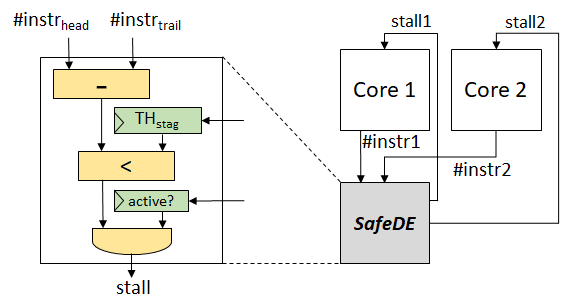
\includegraphics[keepaspectratio,width=\columnwidth]{img/safede}
        \caption{Simplified light-lockstep scheme with SafeDE.}
	\label{fig:simplified_scheme}
\end{figure}
In figure \ref{fig:simplified_scheme} it is shown a simplified light-lockstep scheme with SafeDE. When active, SafeDE counts the instructions executed by both cores. Each cycle, SafeDE computes the staggering substrating those instructions executed by the trail core to the ones executed by the head core. If that difference (staggering) is smaller than a given threshold, the trail core is stalled.

A light-lockstep execution implemented with SafeDE offers some advantages in contrast with the classical lockstep approach:
\begin{itemize}
	\item \textbf{Low-cost:} SafeDE employs few hardware resources.
	\item \textbf{Flexibility:} SafeDE can be enabled and disable at will. This allows the possibility of using a couple of cores to execute either two tasks with SafeDE disabled or one task with SafeDE enabled, depending on its criticality.
        \item \textbf{Low intrusiveness:} SafeDE can be implemented in a SoC performing only a few modifications in the design. Namely, SafeDE needs only the instruction counters and two signals to stall the cores. 
\end{itemize}

When working in light-lockstep mode, both cores have to execute exactly the same instructions so that software does not diverge. For that reason, they need to execute redundant independent processes allocated in different segments of memory. Even though SafeDE guarantees time diversity, a software mechanism to detect the discrepancies in the results of both cores has to be implemented. SafeDE is devised to work in bare metal since an operating system could make the paths of the redundant cores diverge (e.g. interruptions, exceptions).

\hspace{5cm}


%----------------------------------------------------------------------------------------
%	Section 2
%----------------------------------------------------------------------------------------

\section{Signal descriptions}

Table \ref{t_ports} shows the interface of the core (VHDL ports).
\begin{table}[H]
	\caption{Signal descriptions (VHDL ports)}
	\label{t_ports}
	\centering
	\begin{footnotesize}
	\begin{tabular}{|l|l|l|p{6cm}|l|}
		\hline
		\textbf{Signal name} & \textbf{Field}  & \textbf{Type}  & \textbf{Function} & \textbf{Active}\\
		\hline
		RSTN & &Input &Reset & Low\\
		\hline
		CLK & &Input &AHB master bus clock & -\\
		\hline
		ICNT1\_I & &Input & Input to count the instructions executed by core1 & High\\
		\hline
		ICNT2\_I & &Input & Input to count the instructions executed by core2 & High\\
		\hline
		STALL1\_O & &Output & Output to stall the pipeline of core1 & High\\
		\hline
		STALL2\_O & &Output & Output to stall the pipeline of core2 & High\\
		\hline
		APBI\_I & * &Input &APB slave output signals, includes interrupts & - \\
		\hline
		APBO\_O & * &Output &APB slave output signals, includes interrupts & - \\
		\hline
	\end{tabular}
\end{footnotesize}
\end{table}

Signals ICNT1\_I and ICNT2\_I come from the pipelines of the cores. These signals have two bits each, one bit per lane. When one instruction is committed in one of the lanes, the corresponding bit will be set to 1 during one cycle.

Signals STALL1\_O and STALL2\_O come from SafeDE to the caches controllers and pipelines of the cores. These signals hold the pipelines of the cores when they are set to 1.

SafeDE is designed to work with two cores. The pair of signals ICNT\_1 and STALL\_1 have to be wired to the pipeline of the same core. This core will be considered the core1 and will have to write the register \ref{critical1} explained in the section \ref{operation_chap}. The same reasoning is applicable to core2.


\hspace{2cm}




\section{Configuration options}
\label{confg_chap}
Table \ref{generics} shows the configuration parameters (VDHL generics) exposed by \textit{apb\_wrapper.vhd}. 
\\
\begin{table}[H]
	\caption{Configuration options (VHDL ports)}
	\label{generics}
	\centering
	\begin{small}
		\begin{tabular}{|l|p{6cm}|l|l|}
			\hline
			\textbf{Generic} & \textbf{Function}  & \textbf{Allowed range}  & \textbf{Default}\\
			\hline
			PADDR  & APB base address &0 to 16\#fff\# & 0\\
			\hline
			PMASK  & APB address mask &0 to 16\#fff\# & 16\#fff\#\\
			\hline
			PINDEX & APB slave index &0 to 16\#fff\# & 16\#fff\#\\
			\hline
			PIRQ   & APB interrupt index &0 to 16\#fff\# & 16\#fff\#\\
			\hline
			LANES\_NUMBER & Lanes of the processor & 1 to 5 & 2\\
			\hline
			REGISTER\_OUTPUT & If set to 1, the STALL outpus are registered to improve timing & 0 or 1 & 0 \\
			\hline
			MIN\_STAGGERING\_INIT & If the minimum staggering threshold is not changed through the software, its value will be this parameter& 5 to 32740 & 20 \\
			\hline
                        EN\_CYCLES\_LIMIT & Maximum number of cycles allowed between setting to 1 one of the critical section registers \ref{critical1} \ref{critical2} and the other before raising an interrupt & ALL & 500 \\
			\hline
		\end{tabular}
	\end{small}
\end{table}

\hspace{2cm}


\newpage
\section{Operation}
\label{operation_chap}
\subsection{General}
SafeDE is controlled through three internal registers:

The output signals used to stall the cores \ref{t_ports} are anded with the bit 30 of the configuration register \ref{cfg0}. If this bit is set to 0, SafeDE will be able to stop neither of the cores. If bit 31 "soft\_reset" is set to 1, all SafeDE registers are set to its reset value except the configuration register. In the same register, there are 15 bits to configure the maximum and the minimum staggering allowed. When the staggering is smaller or bigger than these thresholds, the trail or the head core will be stalled until the staggering is within limits again. If the value of "max\_staggering" is kept to 0, the value of the maximum staggering will be 32750 to avoid overflows. If "min\_staggering" is kept to 0, the value of the maximum staggering will be the value of the VHDL generics min\_staggering\_init explained in table \ref{generics}.

\begin{register}{H}{SafeDE configuration register 0}{0x00}
	\label{cfg0}
	\regfield{Soft\_reset}{1}{31}{{0}}
	\regfield{Global\_enable}{1}{30}{{0}}
	\regfield{max\_staggering}{15}{15}{{0}}
	\regfield{min\_staggering}{15}{0}{{0}}
	\reglabel{Reset value}\regnewline
\end{register}

To choose the correct value for maximum and minimum staggering is important to take into account the configurations options in section \ref{confg_chap}. If SafeDE is configured to work with a two-lanes core, it means that in each cycle, two instructions can be committed. If we choose a minimum staggering of 15 instructions, that means that each time that the staggering is equal to or smaller than 15, the trail core will be stalled. However, at some point, the staggering could be 16, and the trail core could commit two instructions. In this scenario, the staggering would become 14, and the minimum staggering threshold would be exceeded. Suppose the VHDL generic "register\_output" in table \ref{generics} is set to 1 for timing issues. In that case, the minimum staggering threshold can be exceeded by three instructions instead of one due to the delay between the assertion of the stall signal and the time that it takes effect in the pipeline. In conclusion, depending on the configuration, the threshold can be exceeded by a few instructions. In case a low minimum staggering threshold is chosen, this could cause SafeDE malfunction if the staggering gets 0 or lower.

Apart from the  configuration register, SafeDE has two other registers \ref{critical1} and \ref{critical2}. The function of these registers is to indicate SafeDE that the core has started the critical task. Each core has assigned one critical section register, and it has to set its first bit before starting the critical section. Once the register is set to '1', SafeDE will start counting the executed instructions by that core. In this way, the instructions are counted starting from the same point. It could happen that the write instruction in the "Critical\_section" register had some delay because of the write buffer. Suppose the write buffers of the two cores are not equally filled when the write instruction is fetched. In that case, both cores could execute a different number of instructions, and the staggering computed by SafeDE could vary some instructions from the real value. This can be avoided by reading the critical section register right after writing it (in the next instruction).

\begin{register}{H}{Critical section 1 register 1}{0x04}
	\label{critical1}
	\regfield{Reserved}{31}{1}{{X}}
	\regfield{Critical\_Section1}{1}{0}{{0}}
	\reglabel{Reset value}\regnewline
\end{register}

\begin{register}{H}{Critical section 2 register 2}{0x08}
	\label{critical2}
	\regfield{Reserved}{31}{1}{{X}}
	\regfield{Critical\_Section2}{1}{0}{{0}}
	\reglabel{Reset value}\regnewline
\end{register}

It doesn't matter which core enters first the critical section (core1 or core2). The first core entering the critical section will take the role of head core and vice-versa. A mechanism also raises an interrupt if one core enters its critical section and the other doesn't. VHDL generic EN\_CYCLES\_LIMIT described in table \ref{generics} determine how many cycles can elapse between one core and the other enter their critical section.





\newpage
\subsection{Statistics}

In addition to the configuration registers, SafeDE also has some registers that store statistics of the execution for debug purpuses. All these registers are shown in figure \ref{fig:reg_statistics}.

\begin{figure}[H]
	\begin{center}
		\regfieldb{0x0c}{32}{0}
		\reglabelb{Total cyles active} \\
		\regfieldb{0x10}{32}{0}
		\reglabelb{Executed instructions core1} \\
		\regfieldb{0x14}{32}{0}
		\reglabelb{Executed instructions core2} \\
		\regfieldb{0x18}{32}{0}
		\reglabelb{Times stalled core1} \\
		\regfieldb{0x1c}{32}{0}
		\reglabelb{Times stalled core2} \\
		\regfieldb{0x20}{32}{0}
		\reglabelb{Cycles stalled core1} \\
		\regfieldb{0x24}{32}{0}
		\reglabelb{Cycles stalled core2} \\
		\regfieldb{0x28}{32}{0}
		\reglabelb{Maximum staggering} \\
		\regfieldb{0x2c}{32}{0}
		\reglabelb{Accumulated staggering} \\
		\regfieldb{0x30}{32}{0}
		\reglabelb{Minimum staggering} \\
		\end{center}
	\caption{Statistics registers}\label{fig:reg_statistics}
\end{figure}

The maximum staggering register (0x28) stores the maximum staggering achieved during the execution. The minimum staggering register (0x30) stores the minimum staggering achieved during the execution. However, this register is only updated once both cores have entered the critical section and the staggering is equal to or bigger than the minimum threshold. Each cycle is added to the value of the Accumulated staggering register (0x2C) the value of the staggering. The average staggering can be derived by dividing the value of this register by the number of cycles active.

All statistic registers except the minimum staggering register are updated once one core has entered its critical section (head core) and until the head core has finished its critical section. To reset these registers, the soft\_reset bit in the configuration register \ref{cfg0} has to be set to 1. None of these registers have any mechanism to prevent overflow.

\hspace{1cm}



\subsection{Software support}

The unit can be configured by the user at a low level following the description of previous sections. In addition we provide a small bare-metal driver under the path \\ \textit{grlib/software/noelv/BSC\_tests/BSC\_libraries/light-lockstep}.

The driver is composed of three files.
\begin{itemize}
\item \textit{lightlock\_vars.h}: Defines a set of constants with the RTL parameters and the memory position of the lockstep within the memory map of the SoC.
\item \textit{lightlock.h}: It contains the prototypes of each function of the driver.
\item \textit{lightlock.c}: Contains the definition of each of the functions.
\end{itemize}

The functions defined in the driver are: 
\begin{itemize}
\item \textit{lightlock\_enable()}: Sets to 1 the 31 bit of the configuration register \ref{cfg0}. It has to be called by any core to make SafeDE work.
\item \textit{lightlock\_disable()}: Sets to 0 the 31 bit of the configuration register \ref{cfg0}. SafeDE won't work independently of the value of the other registers. 
\item \textit{lightlock\_min\_threshold(int min\_threshold)}: It changes the value of the minimum staggering threshold. 
\item \textit{lightlock\_min\_max\_thresholds(int min\_threshold, max\_threshold)}: It changes the value of the minimum and the maximum staggering thresholds.
\item \textit{lightlock\_start\_criticalSec(int core)}: It has to be called right before entering the critical section. The argument of the function must be 1 or 2, for core1 or core2 respectively.
\item \textit{lightlock\_finish\_criticalSec(int core)}: It has to be called right after finishing the critical section. The argument of the function must be 1 or 2, for core1 or core2 respectively.
\item \textit{lightlock\_report()}: It prints the values stored in the statistic registers.
\item \textit{lightlock\_softreset()}: It resets all the registers in the module except the configuration register \ref{cfg0}.
\end{itemize}


\hspace{2cm}


\section{Library dependences}
Table \ref{dep_tab} shows the VHDL libraries used when instantiating SafeDE.\\
%%TODO: check if the libraries are actually needed
\begin{table}[H]
	\caption{Library dependencies}
	\label{dep_tab}
	\centering
		\begin{small}
	\begin{tabular}{|l|l|l|l|}
		\hline
		\textbf{Library} & \textbf{Package}  & \textbf{Imported units}  & \textbf{Description} \\
		\hline
		IEEE & std\_logic\_1164 & Types & Standard logic types\\
		\hline
		IEEE & numeric\_std & Functions and types & Arithmetic functions and signed and unsigned types\\
		\hline
		IEEE & math\_real & Constants and functions & Mathematical functions and constants\\
		\hline
		GRLIB & amba & Signals & AMBA signal definitions\\
		\hline
		GRLIB & devices  & Types  & Device names and vendors \\
		\hline
		BSC & ligthlock\_pkg & Instances and signals & Instances and type definitions for SafeDE\\
		\hline
		BSC & lightlock\_module & Instance & Instance of SafeDE top module\\
		\hline
	\end{tabular}
\end{small}
\end{table}


\hspace{2cm}


\section{Instantiation}
An example design is provided in the context of De-RISC.
\\
\belowcaptionskip=-10pt
\begin{lstlisting}[label=ins-prot,caption=SafePMU instance example for gpp\_sys,style=vhdl]
-- Include BSC library
library bsc;
use bsc.lightlock_module.all;

--Provide non-overlaping APB parameters
constant psidx_safede : integer := 5;
constant paddr_safede : integer := 6;
-- Chose minimum length: 256 bytes;
constant pmask_safede : integer := 16#fff#;  
constant pirq_safede : integer := 14;

--Declare signals with as many bits as lanes are.
--Each bit of each lane has to be set to '1' during one 
--cycle when one instruction is commited in that lane
singal icnt1 : std_logic_vector(1 downto 0);
singal icnt2 : std_logic_vector(1 downto 0);

--Declare signals that are able to stall the pipelines
signal lockstep_stall1 : std_logic;  -- For core1
signal lockstep_stall2 : std_logic;  -- For core2


--Instance of the unit
apb_lockstep_inst : apb_wrapper_lockstep
  generic map(
      pindex    => psidx_safede,
      paddr     => paddr_safede,            
      pmask     => pmask_safede,
      pirq      => pirq_safede,
      lanes_number        => 2,
      register_output     => 0,
      register_input      => 0,
      en_cycles_limit     => 500,
      min_staggering_init => 20
      )
  port map(
      rstn     => rstn,
      clk      => clkm,
      apbi_i   => apbi(psidx_safede),
      apbo_o   => apbo(psidx_safede),
      icnt1_i  => icnt1, 
      icnt2_i  => icnt2, 
      stall1_o => lockstep_stall1,
      stall2_o => lockstep_stall2
      );

\end{lstlisting}

\end{document}



\section{Special cases, corner cases}

After reset of a top module (PMU\_raw for instance) you may experience that all the outputs route the event in the first position of vector\_i. This is intended behavior and happens due to the reset of the configuration registers (cfg\_i).\\
\\
In the default integration with PMU\_raw.sv there is a self-test capability that bypasses the crossbar with certain test patterns. This \textbf{self-test capability} is configured in the main configuration register of PMU\_raw.sv. Be sure to have this function disabled if you plan to use the crossbar.





\end{document}
